\documentclass{article}

% if you need to pass options to natbib, use, e.g.:
% \PassOptionsToPackage{numbers, compress}{natbib}
% before loading nips_2017
%
% to avoid loading the natbib package, add option nonatbib:
% \usepackage[nonatbib]{nips_2017}

\usepackage[final]{nips_2017}

% to compile a camera-ready version, add the [final] option, e.g.:
% \usepackage[final]{nips_2017}

\usepackage[utf8]{inputenc} % allow utf-8 input
\usepackage[T1]{fontenc}    % use 8-bit T1 fonts
\usepackage{hyperref}       % hyperlinks
\usepackage{url}            % simple URL typesetting
\usepackage{booktabs}       % professional-quality tables
\usepackage{amsfonts}       % blackboard math symbols
\usepackage{nicefrac}       % compact symbols for 1/2, etc.
\usepackage{microtype}      % microtypography
\usepackage{graphicx}
\usepackage{natbib}

\graphicspath{{figures/}}

\title{Cracking Neural Network Hashes with Adversarial Examples}

% The \author macro works with any number of authors. There are two
% commands used to separate the names and addresses of multiple
% authors: \And and \AND.
%
% Using \And between authors leaves it to LaTeX to determine where to
% break the lines. Using \AND forces a line break at that point. So,
% if LaTeX puts 3 of 4 authors names on the first line, and the last
% on the second line, try using \AND instead of \And before the third
% author name.

\author{
  Conrad ~Christensen\\
  Deep Learning, Spring 2018\\
  New York University\\
  \href{mailto:conradbc@cims.nyu.edu}{\texttt{conradbc@cims.nyu.edu}} \\
  \And
  Da ~Ying\\
  Deep Learning, Spring 2018\\
  New York University\\
  \href{mailto:dy877@nyu.edu}{\texttt{dy877@nyu.edu}}
}

\begin{document}
% \nipsfinalcopy is no longer used

\maketitle

\begin{abstract}
    Success of neural networks have lead to a wide range of applications, some
    more appropriate than others. Due to a potential for parallelization, and
    ease of implementation, some works have suggested using neural networks as
    hash functions.  We believe this is a bad idea in terms of security, as
    neural networks are differentiable, which allows methods for collision
    search. We show that it is possible to generate hash collisions for some of
    the basic neural network hash functions. Additionally we explore the
    applicability of multiple techniques from adversarial example generation on
    generating collisions for a neural network hashing algorithm, comparing
    their efficacy.
\end{abstract}

\section{Introduction}
In computer security a cryptographic hash function is a function used to
reduced documents into a fixed size hash (often times represented by a
hexadecimal string).  The application for these range from download document
verification, to storage of passwords \cite{crypoHash}. One of the definiong
properties of this class of functions is that they are one-way. This means that
given a hash of a document, it is infeasible to find a document (a hash
collision) that produces the same hash (whether it is the same as the original
or not) \cite{crypoHash}.  This is particularly import if a company stores
password hashes. If these are lost to an adversary, it is important that the
adversary cannot find another password that produces the same hash, as then
they could use this to authenticate as one of the users.

There has been a recent increase in using machine learning to solve, or as part
of a solution, to systems problems. For example in \cite{learnedIndex}, the
authors use neural networks to learn the index distribution for data storage,
to replace B-Trees indexes for data retrieval. The problem of finding good
cryptographic using neural networks has also been proposed in multiple papers
\cite{hash1, hash2}. In this work we show that these hash functions
fundamentally do not satisfy the one-way requirement for cryptographic hashes,
as they expose sensitive information through the gradients of the network that
can be exploited to find hash collisions.

\section{Related Work}

Related to our approach of using the gradients of a neural network to alter
the input, is the work of finding adversarial examples that when fed to a
neural network, produce an unexpected output classification \cite{intriguing}.

This idea was first popularized in the work \cite{intriguing}; other methods
for generating these examples soon followed \cite{explaining}; and even defenses
for neural networks against being susceptible to these attacks emerged, such
as \cite{robust, ensemble, distil}. While effective to some degree, it was shown
in \cite{space} that adversarial examples exist in a large number of dimensions
of the input space, suggesting they may be a problem on a more fundamental 
level.

Neural network popularity has led to many unique uses for them. Some in already
solved domains. In \cite{hash1} an RNN is used to process data and produce
a fixed length hash value. This work measured the entropy of the hash function
by how many digits in the hash hexadecimal code were changed. Other authors,
including \cite{hash2} have also proposed using neural networks to create
one-way hash functions.

\section{Neural Hash Function}

The model that we will be attacking here, for the purpose of demonstrating issues 
with neural network cryptographic hash functions, is that described in \cite{hash1}.

%%% Separate image locations
%\begin{figure}[t]
    %\centering
    %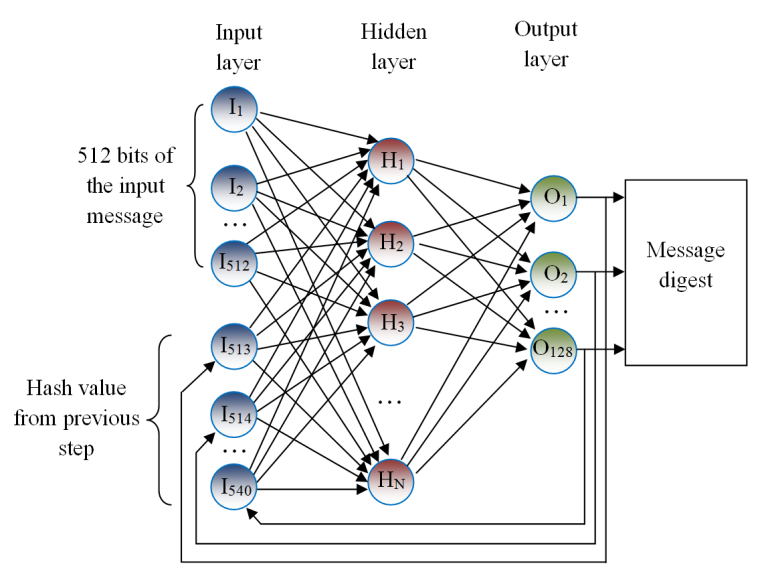
\includegraphics[width=90mm]{hash_nn_architecture}
    %\caption{A simple caption} 
    %\label{fig:hashNN}
%\end{figure}

%\begin{figure}[b]
    %\centering
    %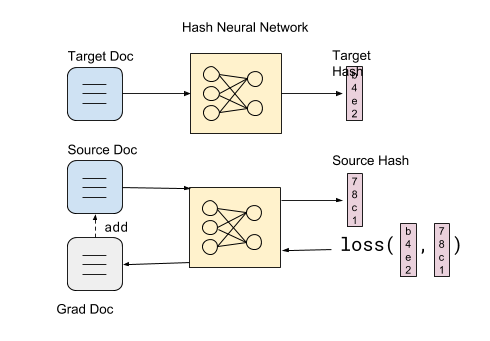
\includegraphics[width=90mm]{model_diagram}
    %\caption{Collision attack overview} 
    %\label{fig:model}
%\end{figure}


%%% Images side-by-side with minipages to save room.
\begin{figure}[t]
    \centering
    \begin{minipage}{.5\textwidth}
        \centering
        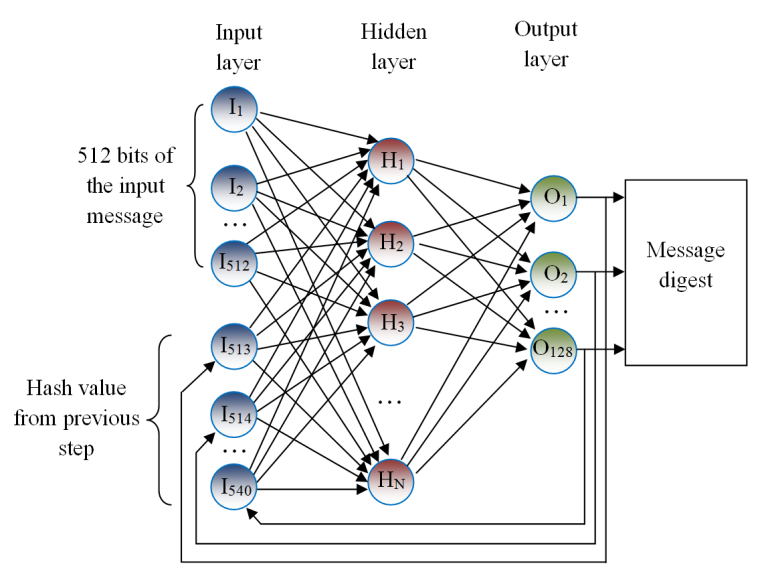
\includegraphics[width=\textwidth]{hash_nn_architecture}
        \caption{Hash function algorithm presented in \cite{hash1}}
        \label{fig:hashNN}
    \end{minipage}%
    \begin{minipage}{.5\textwidth}
        \centering
        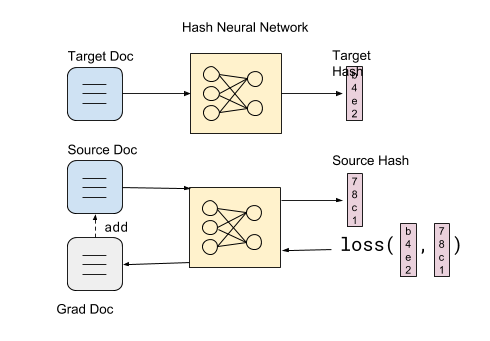
\includegraphics[width=\textwidth]{model_diagram}
        \caption{Collision attack overview} 
        \label{fig:model}
    \end{minipage}
\end{figure}



Look at the nn hash figure in Figure \ref{fig:hashNN}.

\section{Attack Approach}

Look at image in Figure \ref{fig:model}.

\section{Results}

\section{Conclusion}

\bibliographystyle{unsrt}
\bibliography{ref} 

\end{document}
